
\chapter{Simulation Studies\label{chap:5}}

This chapter focuses on studying the methods proposed in the previous
two chapters in a simulation environment. 


\section{Sampling $\nu$-bridges}

In this first section, we demonstrate that the exact generalized bridge
sampler proposed in \chapref{4} produces samples from the desired
target distribution. Furthermore, we show that both the approximate
and exact samplers are robust to the specific conditions imposed on
the nature of the stochastic process to be bridged in \chapref{2}.
We also confirm that the approximate sampler does not formally draw
from the true generalized bridge distribution, but note that the approximate
sample paths are still qualitatively similar to exact sample paths.

As usual, we first fix the objects of study. Though the theoretical
results in \chapref{4} characterize a generalized bridge sampler
for the specific case of It� diffusions with finite speed measure,
we will consider a more general class of processes in this section
to demonstrate the broad applicability of the proposed generalized
bridge samplers. In particular, we will focus on L�vy processes of
the form 
\begin{equation}
dX_{t}=-\lambda\left(X_{t}-\mu\right)dt+\sigma dL_{t},\label{eq:ou-sde}
\end{equation}
for some initial condition on $X_{0}$ and L�vy process $L$, where
$\lambda,\sigma>0$. Solutions to this SDE are known as L�vy-driven
Ornstein-Uhlenbeck (OU) processes. When $L$ is a Wiener process,
$X$ is an It� diffusion satisfying the assumptions outlined in \chapref{2}.
This so-called Gaussian OU process, or OU diffusion, is both theoretically
interesting (representing the only non-trivial stationary, Gaussian,
and Markovian process) and practically useful as a model for a wide
range of processes (see \citet[Section 1.2 in][]{hirsa-2012} for
applications in finance, for instance). In general, we will refer
to the parameter vector of such a process as $\theta=(\mu,\lambda,\sigma)$,
and the joint law at $\mathcal{T}=\{0,1\}$ of a solution to (\ref{eq:ou-sde})
with initial condition $X_{0}\sim F$ as $\nu_{\theta}(F,L)$. 

In all simulations to be carried out, the relevant process is simulated
over the time interval $[0,1]$ with step size $\delta=1/100$ using
the Euler-Maruyama scheme. In this section, we will repeatedly need
to sample from $\nu_{\theta}(F,L)$; this can be easily done by simulating
an unconstrained solution to (\ref{eq:ou-sde}) with initial condition
$X_{0}\sim F$, and taking its values at $\mathcal{T}=\{0,1\}$. The
exact generalized bridge sampler uses $M=10$ (the number of $T$-values
simulated in order to calculate $\hat{\rho}$).

\begin{table}[t]
\centering \begin{tabular}{@{}lllllll@{}} \toprule \multirow{2}{*}{\parbox{2cm}{Process \& Initial Dist.}} & \multicolumn{2}{l}{K-S stat. ($\times 10^{-2}$)} && \multicolumn{2}{l}{CPU (rel.)} \\ \cmidrule(l){2-3} \cmidrule(l){5-6}                                    & Approx.                   & Exact                  && Approx.                  & Exact                 \\ \midrule \emph{OU (Gaussian)}             &                           &                        &&                          &                       \\ \:\:\:\:$\mathcal{N}(0,1/2)$               & 2.17*                     & 1.62           &        & 2.74                      & 76.7                  \\ \:\:\:\:$2\text{Bern}-1$                   & 3.08***                   & 1.11            &       & 3.35                      & 94.7                  \\ \:\:\:\:$\text{Expo}$                      & 3.12**                    & 1.95             &      & 2.94                      & 96.3                  \\ \emph{OU ($\alpha$-stable)}             &                           &                      &  &                          &                       \\ \:\:\:\:$\mathcal{N}(0,1/2)$               & 2.30*                     & 1.39               &    & 3.47                      & 85.9                  \\ \:\:\:\:$2\text{Bern}-1$                   & 2.26*                      & 1.58               &    & 5.08                      & 93.5                  \\ \:\:\:\:$\text{Expo}$                      & 3.85***                   & 2.75**               &  & 4.32                      & 97.5                  \\ \emph{Wiener}             &                           &                        &               &           &                       \\ \:\:\:\:$\mathcal{N}(0,1/2)$               & 0.97                      & 0.69                  & & 4.01                      & 77.8                  \\ \:\:\:\:$2\text{Bern}-1$                   & 1.54                     & 0.09                   && 3.92                      & 72.2                  \\ \:\:\:\:$\text{Expo}$                      & 1.60                      & 0.89                  & & 4.88                      & 76.2                  \\
\bottomrule \end{tabular}


\begin{centering}
\begin{tabular}{lllll>{\raggedright}m{2cm}}
\multirow{1}{*}{} & \multirow{1}{*}{} &  &  &  & \tabularnewline
\end{tabular}
\par\end{centering}

\caption{\label{tab:KS-stats}Kolmogorov-Smirnov (K-S) statistics comparing
$10,000$ sample paths at $t=1/2$ of solutions $X$ to (\ref{eq:ou-sde})
against approximately and exactly generalized bridges of $X$. The
running times relative to sampling the unconstrained processes are
also presented. $*,**,***$ denote statistically significant K-S statistics
at the $95\%,99\%,$ and $99.9\%$ confidence levels.}
\end{table}


Now, note that an unconstrained solution to (\ref{eq:ou-sde}) with
initial condition $X_{0}\sim F$ can be equivalently viewed as its
own $\nu_{\theta}(F,L)$-bridge. This insight suggests that we merely
need to verify that a $\nu_{\theta}(F,L)$-bridge of $X$ is equal
in distribution to the unconstrained process $X$ when $X_{0}\sim F$.
In \tabref{KS-stats}, we present Kolmogorov-Smirnov (K-S) statistics
comparing the marginal distribution at $t=1/2$ of unconstrained processes
to their $\nu_{\theta}(F,L)$-bridges sampled approximately and exactly.
The relative running times of the two samplers are also given. A significant
K-S statistic says that we may reject the null hypothesis that the
samples being compared are drawn from the same distribution at some
appropriate confidence level. 

In addition to evaluating the correctness of the proposed generalized
bridge samplers for a Gaussian OU process with $\theta=(0,1,1)$,
which satisfies the assumptions of \chapref{2}, we also test the
correctness of the samplers for 
\begin{aenumerate}
\item an OU process driven by a standard $\alpha$-stable L�vy process $L_{\alpha}$
with $\theta=(0,1,1)$, which is not an It� diffusion, and 
\item the Wiener process, which does not have finite speed measure. 
\end{aenumerate}
Note the Wiener process is a limiting case of the Gaussian OU process
when $\theta\rightarrow(0,0,1)$. For each process, we evaluate the
quality of the sampled bridges for $F$ equal to
\begin{aenumerate}
\item $\mathcal{N}(0,1/2)$, the stationary distribution of a Gaussian OU
process with $\theta=(0,1,1)$,
\item $2\mbox{Bern}-1$, a discrete distribution, and
\item $\mbox{Expo}$, a distribution with relatively heavy tails (where
the log-density decays linearly instead of quadratically like the
Gaussian distribution).
\end{aenumerate}
\tabref{KS-stats} confirms that for the OU diffusion, we cannot reject
the null hypothesis that the exact sampler draws from the true distribution
at the $95\%$ confidence level for a variety of initial distributions.
On the other hand, we can reject the null hypothesis for the approximate
sampler at the same confidence level; this is expected, since \thmref{approx-sim}
says explicitly that the approximate sampler for an It� diffusion
draws generalized bridges conditional on such bridges being hit by
an independent hitting diffusion. 

We note that the quality of the approximate sampler is inversely correlated
with the computing time required to sample exact bridges. This intuitively
highlights a tradeoff between speed and quality, and is also formally
expected: If the approximate sampler produces low quality samples,
then their probability of intersection with a hitting diffusion is
low. Since the exact sampler accepts, with high probability, sample
paths that are less likely to intersect with a hitting diffusion,
it must spend more time simulating hitting diffusions for any given
proposal.

The bridges produced by the exact sampler for the $\alpha$-stable
OU and Wiener processes also appear to be generally of high quality,
suggesting that the proposed method is fairly robust to the assumptions
made in \chapref{2}. It is only in the extreme case of an $\mbox{Expo}$
initial distribution and an $\alpha$-stable L�vy-driven OU process
that the exact sampler fails to draw from the true bridge distribution
at $t=1/2$. We conjecture that the infinite variance of the innovations
of the process and the relatively heavy tail of the initial distribution
dramatically reduce the probability of intersection with a mean reverting
hitting process. In particular, our choice of $M=10$ Monte Carlo
samples for estimating the hitting probability may result in Metropolis-Hastings
acceptance ratios that are too coarse to produce exact paths in a
finite sample scenario.

Unexpectedly, both the approximate and exact samplers appear to sample
from the true bridge distribution when the underlying process is a
Wiener process, which does not have finite speed measure. We do not
have a theoretically grounded explanation for this phenomenon; however,
we see this result as further evidence that the assumptions made in
\chapref{2} regarding the sorts of processes that can be bridged
may be relaxed in future research.

\begin{figure}[t]
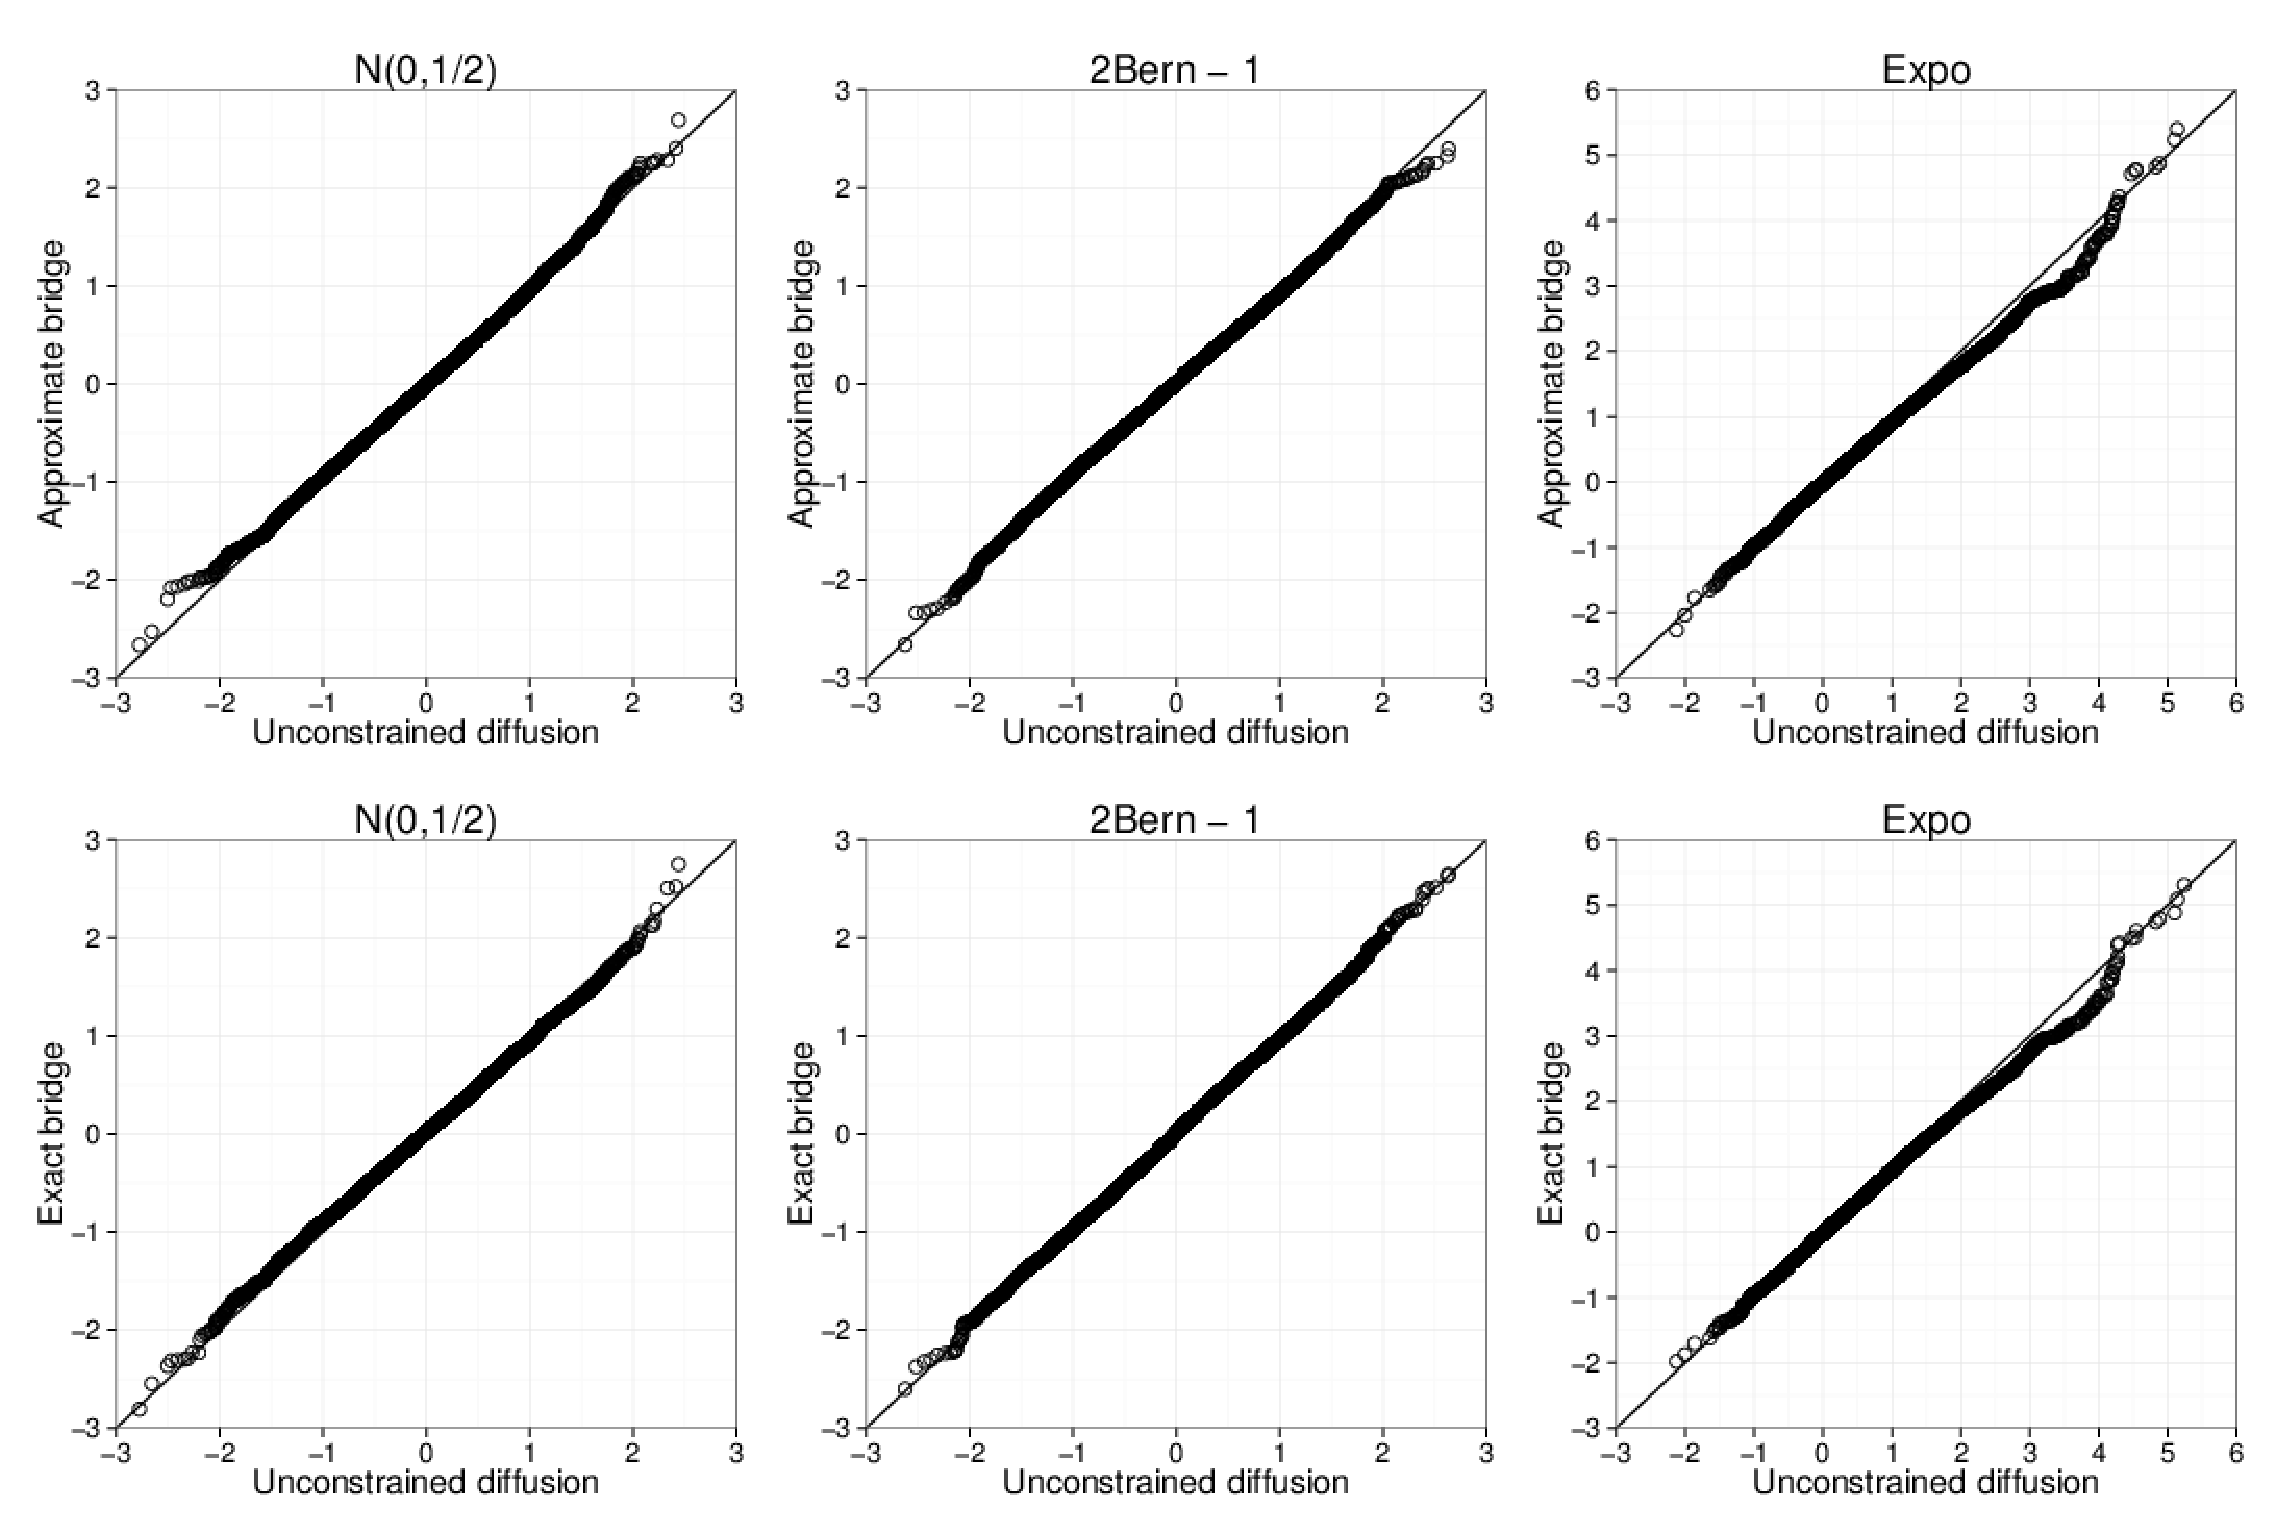
\includegraphics[width=1\columnwidth]{/Users/marshall/Documents/senior/thesis/figures/approx-vs-exact}

\caption{\label{fig:q-q}Q-Q plots comparing $10,000$ sample paths at $t=1/2$
of an unconstrained Gaussian OU process $X$ governed by $\theta=(0,1,1)$
to the corresponding approximate and exact $\nu_{\theta}(F,W)$-bridges
of $X$, for $F\sim\mathcal{N}(0,1/2),$ $F\sim2\mbox{Bern}-1$, and
$F\sim\mbox{Expo}$. }
\end{figure}


While it is true that the approximate sampler does not formally sample
from the true generalized bridge distribution, we show in \figref{q-q}
that the approximate and exact samplers for the Gaussian OU bridges
produce qualitatively similar samples. In general, we see that the
approximate samples are slightly thinner-tailed than the true distribution:
This is expected, since conditional on the approximate samples being
hit by a hitting process (which in this case mean-reverts to $0$),
the approximate sample paths should tend toward $0$ as well. \figref{q-q}
reveals that $F\sim\mbox{Expo}$ results in the lowest quality samples,
whether from the approximate or exact sampler (corroborating the high
K-S statistics observed in \tabref{KS-stats}). The values around
$3.5$ which deviate substantially from the true distribution can
be understood as coming from the sample paths which were initialized
at extreme values, but which have since mean reverted towards $0$.
We hypothesize that the exact sampler has difficulty correcting these
paths because the coarse estimates used for the M-H acceptance ratios
cannot capture their low probability of intersection with a mean reverting
hitting process, as described above.

In light of the qualitative similarity of the approximate and exact
samplers, it is worth noting that the K-S statistics presented in
\tabref{KS-stats} represent the most liberal estimates of deviation
from the true distribution. In particular, $t=1/2$ represents the
point in time at which the marginal distributions of these bridges
have the most freedom to deviate from the true distribution (in contrast,
the marginal distribution of the sampled bridges, whether approximate
or exact, are the same as the unconstrained process at times $\mathcal{T}=\{0,1\}$
by definition). The K-S statistics presented here are therefore an
overly stringent view of the utility of the approximate sample paths
in the MCEM algorithm proposed in \chapref{EM}. In particular, the
proposed MCEM algorithm depends on an integral over an entire generalized
bridge path, and not only on the value of a bridge at $t=1/2$. In
the next section, we will demonstrate that an MCEM algorithm using
the approximate bridge sampler produces comparable results to one
using the exact bridge sampler, and demonstrate the correctness of
the proposed MCEM algorithm more generally.


\section{Simulation-Based Inference on Distributional Data}

Having verified our ability to sample $\nu$-bridges, we verify in
this section the correctness of the MCEM algorithm proposed in \chapref{EM}.
We show that the MCEM scheme converges to the Kullback-Liebler divergence
minimizing parameter in a variety of settings, often very quickly.
Furthermore, we demonstrate that using an approximate generalized
bridge sampler does not seem to adversely affect convergence up to
Monte Carlo variation. Given that the approximate sampler is one to
two orders of magnitude faster than the exact sampler (as seen in
\tabref{KS-stats}), this is a welcome finding that dramatically increases
the utility of the proposed MCEM scheme in inference applications.

The theoretical setting for this section is as follows: Suppose we
have an true but unknown probability model $\mathbb{P}$ admitting
a canonical process $X$ on the interval $[0,1]$. Further suppose
we wish to model $X$ under a family of alternative probability models
$\mathcal{Q}=\{\mathbb{Q}_{\theta}\mid\theta\in\Theta\}$, where $\mathbb{P}$
is absolutely continuous to any element of $\mathcal{Q}$. $X_{0}=x_{0}$
is fixed in either model, and we let $\nu_{\mathbb{P}}$ be the known
law of $X$ under $\mathbb{P}$ at times $\mathcal{T}=\{t_{1},\dots,t_{n}\}$,
where $t_{1}>0$ and we choose $n\geq2$ for identifiability reasons. 

In this section, we will focus on the family of models $\mathcal{Q}$
under which $X$ is a Gaussian OU process. This is due to the prevalence
of such processes as discussed above and the analytical tractability
of the K-L divergence of their finite-dimensional distributions from
those of other Gaussian processes.

Our simulation strategy rests on the following observation: If we
can simulate $X$ under $\mathbb{P}$ on the interval $[0,1]$, we
can take its values at $\mathcal{T}$ as samples from $\nu_{\mathbb{P}}$;
then, the proposed MCEM scheme given $\nu_{\mathbb{P}}$ should converge
to the $\theta$ which minimizes the K-L divergence of the law of
$X$ under $\mathbb{Q}_{\theta}$ from its law under $\mathbb{P}$.
If $X$ is an OU diffusion with parameter $\theta^{*}$ under $\mathbb{P}$,
this K-L divergence minimizing parameter is simply $\theta^{*}$.
Otherwise, so long as $X$ is a Gaussian process under $\mathbb{P}$,
the K-L divergence of any finite-dimensional distribution of $\mathbb{Q}_{\theta}\in\mathcal{Q}$
from the corresponding distribution of $\mathbb{P}$ is analytically
available.

In all simulations to be carried out, the relevant process is simulated
over the time interval $[0,1]$ with step size $\delta=1/100$ using
the Euler-Maruyama scheme. $\mathcal{T}$ is fixed to be $\{1/2,1\}$.
The exact generalized bridge sampler uses $M=10$ as before, and all
optimizations are carried out using the \texttt{R} package \texttt{DEoptim}
(differential evolution optimization) developed by \citet{deoptim}
on default settings and optimization strategy 6. Ten expectation-maximization
iterations in every replication of the MCEM algorithm are performed.
We will refer to MCEM schemes using exactly sampled bridges and approximately
sampled bridges as exact MCEM and approximate MCEM respectively.

\begin{table*}[t]

\centering \begin{tabular}{@{}clcccccccccc@{}} \toprule \multirow{2}{*}{$i$} &  & \multicolumn{3}{l}{Approx.}                                                                                 && \multicolumn{3}{l}{Exact}                                                                                           \\ \cmidrule(lr){3-5}\cmidrule(lr){7-9}                             &  & \multicolumn{1}{c}{$\hat{\mu}$} & \multicolumn{1}{c}{$\hat{\lambda}$} & \multicolumn{1}{c}{$\hat{\sigma}$}  &   & \multicolumn{1}{c}{$\hat{\mu}$} & \multicolumn{1}{c}{$\hat{\lambda}$} & \multicolumn{1}{c}{$\hat{\sigma}$} \\ \cmidrule(r){1-1} \cmidrule(lr){3-9} 0                          &  & 2.00                                & \:2.00\:                        & \:2.00\:                            && \:2.00\:                            & \:2.00\:                           & \:2.00\:                       \\ 1                          &  & 0.59                                & 1.94                            & 1.10                                && 0.10                                & 0.93                               & 0.89                   \\ 2                          &  & 0.06                                & 0.95                            & 0.97                                && 0.01                                & 0.87                               & 0.88    \\ 3                          &  & -0.06\:                               & 1.28                            & 1.07                              & & -0.02\:                            & 0.71                               & 0.88   \\ 4                          &  & 0.18                                & 0.98                            & 0.86                                && -0.10\:                             & 0.97                               & 0.93     \\ 5                          &  & 0.00                                & 1.03                            & 0.95                                && 0.02                                & 0.98                               & 0.98  \\ 6                          &  & 0.02                                & 0.94                            & 0.88                                && 0.04                                & 1.09                               & 0.99  \\ 7                          &  & 0.01                                & 1.33                            & 0.96                                && -0.03\:                                & 1.19                               & 1.06    \\ 8                          &  & -0.05\:                               & 0.91                            & 1.02                              &  & 0.04                                & 1.01                                  &1.01  \\ 9                          &  & 0.01                                & 1.01                            & 0.99                                && 0.04                                & 1.04                                   & 0.99 \\ 10                         &  & -0.04\:                               & 1.04                            & 1.04                              &  & 0.01                                & 1.08                             & 1.01          \\ \bottomrule \end{tabular}

\begin{centering}
\begin{tabular}{lllll>{\raggedright}m{2cm}}
\multirow{1}{*}{} & \multirow{1}{*}{} &  &  &  & \tabularnewline
\end{tabular}
\par\end{centering}

\caption{\label{tab:mcem-stationary}One illustrative replication of exact
and approximate MCEM (using $100\times\left\lfloor i^{1.2}\right\rfloor $
MC samples) to estimate the MKLDE for a Gaussian OU process given
$\nu_{\mathbb{P}}$ where $X$ is a Gaussian OU process governed by
$\theta^{*}=(0,1,1)$ under $\mathbb{P}$.}
\end{table*}


As a first illustrative example, we choose $\mathbb{P}$ such that
$X$ is an OU diffusion governed by the parameters $\theta^{*}=(0,1,1)$
under $\mathbb{P}$. The expectation-maximization iterations of a
single replication of the proposed MCEM algorithm given $\nu_{\mathbb{P}}$
are presented in \tabref{mcem-stationary}. As noted above, we expect
the MCEM estimates to converge to $\theta^{*}$. Since the OU diffusion
has a constant diffusion coefficient, the corresponding Lamperti transform
is $\eta_{\theta}(x)=x/\theta$, and the requisite functions for MCEM
are readily available from the results in \chapref{EM}. 

We qualitatively note from \tabref{mcem-stationary} that the exact
and approximate MCEM schemes converge quite quickly, with no obvious
difference between the schemes up to Monte Carlo variation. As is
usual for MCEM, the algorithm produces parameter estimates sampled
from some neighborhood of the true parameter value as described in
\citet[Section 3.1 in][]{wei-tanner-1990}, instead of converging
deterministically to such a value. Though we expected the slightly
thinner tails of the sample paths drawn in approximate MCEM to result
in some deterioration of the quality of the Monte Carlo estimates,
the Monte Carlo variation in this experiment renders any bias undetectable
to the eye.

With a heuristic sense of the dynamics of the MCEM algorithm's convergence,
we present a comprehensive evaluation of the ability of the proposed
algorithm to estimate the parameters governing a Gaussian OU diffusion
given a variety of $\mathbb{P}$ in \tabref{diff-diffusions}. In
particular, we consider true probability models $\mathbb{P}$ under
which $X$ is
\begin{aenumerate}
\item an OU diffusion governed by $\theta^{*}$, 
\item a standard Wiener process, and 
\item a fractional Wiener process with Hurst parameter $H=0.2$.
\end{aenumerate}
When $X$ is an OU diffusion under $\mathbb{P}$, as noted above,
the MCEM algorithm should simply converge to $\theta^{*}$ since the
family of probability models $\mathcal{Q}$ is correctly specified.
In the latter two cases, model misspecification means that the MCEM
algorithm can only minimize the K-L divergence of the law of $X_{\mathcal{T}}$
under $\mathbb{Q}_{\theta}$ from its law under $\mathbb{P}$ to some
non-zero quantity. When $X$ is a Wiener process under $\mathbb{P}$,
the K-L divergence is minimized as $\lambda\rightarrow0,\sigma\rightarrow1$,
since the OU diffusion reduces to a Wiener process in such a limit
(note $\mu$ in this case is not well-defined). Finally, when $X$
is a fractional Wiener process with Hurst parameter $H$ under $\mathbb{P}$,
the K-L divergence of the law of $X_{1/2,1}$ under $\mathbb{Q}_{\theta}$
from its law under $\mathbb{P}$ can be found to be
\[
\frac{1}{2}\left[\mbox{Tr}\left(\Sigma_{O}(\theta)^{-1}\Sigma_{F}(H)\right)+\log\frac{\det\Sigma_{O}(\theta)}{\det\Sigma_{F}(H)}-2\right],
\]
where
\[
\Sigma_{O}(\theta)=\frac{\sigma^{2}}{2\lambda}\begin{bmatrix}1-e^{-\lambda} & e^{-\lambda/2}-e^{-3\lambda/2}\\
e^{-\lambda/2}-e^{-3\lambda/2} & 1-e^{-2\lambda}
\end{bmatrix},\Sigma_{F}(H)=\begin{bmatrix}2^{-2H} & 1/2\\
1/2 & 1
\end{bmatrix}
\]
are the covariance matrices of the values of an OU diffusion and a
fractional Wiener process with Hurst parameter $H$ at times $\mathcal{T}=\{1/2,1\}$,
respectively. We choose $H=0.2$ so that the fractional Wiener process
that mean reverts (preventing $\lambda$ from binding at $0$), and
numerically find the K-L divergence minimizing parameter to be approximately
$(0.00,0.83,1.45)$.

In addition to varying $\mathbb{P}$, we also test the performance
of the proposed MCEM scheme when we only have access to a finite set
of samples from $\nu_{\mathbb{P}}$. In particular, we draw $100$
samples from $\nu_{\mathbb{P}}$ in each relevant experiment, and
take the resulting empirical distribution $\hat{\nu}_{\mathbb{P}}$
of the samples as a plug-in estimate for $\nu_{\mathbb{P}}$. As noted
in \chapref{EM}, $(X_{\mathcal{T}},\hat{\nu}_{\mathbb{P}})$ is not
a valid Baudoin conditioning since $\hat{\nu}_{\mathbb{P}}$ is not
absolutely continuous to the law of $X_{\mathcal{T}}$ under any element
of $\mathcal{Q}$; however, since the MKLDE given $\hat{\nu}_{\mathbb{P}}$
is consistent for the MKLDE given $\nu_{\mathbb{P}}$, we heuristically
expect the MCEM scheme given $\hat{\nu}_{\mathbb{P}}$ to still produce
accurate (though perhaps less efficient) estimates for the MKLDE given
$\nu_{\mathbb{P}}$.

It is worth pointing out before we examine in detail the results in
\tabref{diff-diffusions} that the reported standard deviations capture
the variability stemming from 

\begin{table}[H]

\centering \begin{tabular}{@{}lccccccc@{}} \toprule \multirow{2}{*}{\parbox{2cm}{Model \& Dist. Data}} & \multicolumn{3}{l}{Approx.} && \multicolumn{3}{l}{Exact}                                          \\ \cmidrule(lr){2-4} \cmidrule(lr){6-8}                          & $\hat{\mu}$                 & $\hat{\lambda}$      & $\hat{\sigma}$       & & $\hat{\mu}$          & $\hat{\lambda}$      & $\hat{\sigma}$       \\ \midrule \emph{OU}              & \multicolumn{1}{c}{\emph{0.00}}        & \multicolumn{1}{c}{\emph{1.00}} & \multicolumn{1}{c}{\emph{1.00}} && \multicolumn{1}{c}{\emph{0.00}} & \multicolumn{1}{c}{\emph{1.00}} & \multicolumn{1}{c}{\emph{1.00}} \\ \:\:\:\:$\nu_\mathbb{P}$               & 0.00                        & 1.00                 & 0.98              &   & -0.00\:                 & 1.00                 & 0.97                 \\ \:\:\:\:\:\:\:\:Std. Dev.                & (0.05)                      & (0.18)               & (0.04)           &    & (0.06)               & (0.26)               & (0.06)               \\ \:\:\:\:$\hat{\nu}_\mathbb{P}$            & 0.01                       & 1.02                & 0.98               &  &        0.00              &    1.03                  &  1.00                    \\ \:\:\:\:\:\:\:\:Std. Dev.                & (0.13)                      & (0.38)               & (0.09)             &  &   (0.05)                   &  (0.35)                    & (0.10)                     \\ 			&&&&&&& \\	 \emph{Wiener}              & \multicolumn{1}{c}{\emph{0.00}}        & \multicolumn{1}{c}{\emph{0.00}} & \multicolumn{1}{c}{\emph{1.00}} && \multicolumn{1}{c}{\emph{0.00}} & \multicolumn{1}{c}{\emph{0.00}} & \multicolumn{1}{c}{\emph{1.00}} \\ \:\:\:\:$\nu_\mathbb{P}$               & -0.13\:                       & 0.08                 & 1.00           &      & 0.00                     & 0.06                     &  0.99                    \\ \:\:\:\:\:\:\:\:Std. Dev.                & (21.0)                      & (0.05)               & (0.03)          &     & (1.83)                      & (0.05)                     &    (0.04)                  \\ \:\:\:\:$\hat{\nu}_\mathbb{P}$            & 0.13                        & 0.15                 & 1.00            &     &    0.05                  &      0.18                &     1.01                 \\ \:\:\:\:\:\:\:\:Std. Dev.                & (3.89)                      & (0.17)               & (0.06)            &   & (3.63)                     & (0.17)                      &  (0.06)                     \\ 			&&&&&&& \\ \emph{Fractional}              & \multicolumn{1}{c}{\emph{0.00}}        & \multicolumn{1}{c}{\emph{0.83}} & \multicolumn{1}{c}{\emph{1.45}} && \multicolumn{1}{c}{\emph{0.00}} & \multicolumn{1}{c}{\emph{0.83}} & \multicolumn{1}{c}{\emph{1.45}} \\ \:\:\:\:$\nu_\mathbb{P}$               & 0.00                        & 0.81                 & 1.43                & &         -0.01\:             &       0.79               &  1.41                    \\ \:\:\:\:\:\:\:\:Std. Dev.                & (0.08)                      & (0.17)               & (0.06)             &  &        (0.15)              &    (0.19)                  &   (0.06)                   \\ \:\:\:\:$\hat{\nu}_\mathbb{P}$            & -0.04\:                       & 0.86                 & 1.45             &    &            0.00          &       0.84               &       1.43               \\ \:\:\:\:\:\:\:\:Std. Dev.                & (0.22)                      & (0.30)               & (0.13)              & &      (0.25)                &   (0.26)                   & (0.09)                     \\ \bottomrule \end{tabular}


\begin{centering}
\begin{tabular}{lllll>{\raggedright}m{2cm}}
\multirow{1}{*}{} & \multirow{1}{*}{} &  &  &  & \tabularnewline
\end{tabular}
\par\end{centering}

\caption{\label{tab:diff-diffusions}Mean and standard deviation of the MKLDEs
obtained from $50$ replications of approximate and exact MCEM for
an OU diffusion, given either $\nu_{\mathbb{P}}$ or the empirical
distribution $\hat{\nu}_{\mathbb{P}}$ induced by $100$ samples from
$\nu_{\mathbb{P}}$, for varying true models $\mathbb{P}$. The true
K-L divergence minimizing parameters are indicated in italics for
each $\mathbb{P}$.}
\end{table}

\begin{aenumerate}
\item the lower bound on the variance of any estimator, 
\item the variance inherent in the Monte Carlo nature of the MCEM algorithm,
and 
\item the variance of the stochastic optimization procedure. 
\end{aenumerate}
As such, the reported standard deviations are larger than they asymptotically
ought to be with a sufficiently large number of MC samples and a sufficiently
precise optimization procedure.

\tabref{diff-diffusions} reveals that both the approximate and exact
MCEM schemes appear to be remarkably accurate for the true minimum
K-L divergence parameter across all experiments, up to a margin of
error equal to the standard deviation of the MKLDEs. We note that
the standard deviation of $\hat{\mu}$ for the Wiener process is in
some cases quite large; this is a result of $\mu$ not being well-defined
when $\lambda=0$. The Wiener process is also the only process for
which the mean MKLDE is greater than a standard deviation away from
the true parameter value; this is because the parameter space of an
OU process is restricted to $\lambda>0$, so estimates for $\lambda$
when $\lambda=0$ will inevitably be biased positively. It is not
clear to us why the estimates for $\lambda$ across all experiments
seem to be much more variable than the estimates for $\mu$ or $\sigma$.
We conjecture that this is a result of continuous diffusion paths
over a compact interval containing infinite information about $\sigma$,
while only containing finite information about the drift parameters
$\mu$ and $\lambda$ (see \citet{nielsen-shephard-2002}); perhaps
in the case of an OU process, it is $\lambda$ in particular for which
information is sparse.

Furthermore, \tabref{diff-diffusions} demonstrates the robustness
of the proposed MCEM scheme to various assumptions. We note that the
finite sample experiments using $\hat{\nu}_{\mathbb{P}}$ as a plug-in
estimator for $\nu_{\mathbb{P}}$ display lower efficiency but remain
accurate despite the violation of technical conditions on the absolute
continuity of $\hat{\nu}_{\mathbb{P}}$ with respect to the elements
of $\mathcal{Q}$. Furthermore, the biased estimates we expected under
approximate MCEM do not appear up to Monte Carlo variation; we hypothesize
that this is due to the approximate sample paths being of high quality
over a sufficiently high proportion of the interval $[0,1]$. 

With the unbiased estimates of approximate MCEM in mind, \tabref{diff-diffusions}
also shows that the exact MCEM scheme also does not appear to have
obviously less variability than the approximate scheme. Furthermore,
as seen in \tabref{KS-stats}, the computational time taken by an
exact MCEM scheme is at least an order of a magnitude greater than
the time needed for approximate MCEM, which itself is already non-trivial
(on the order of five hours for the experiments shown here, mostly
due to the numerous evaluations of the objective function needed for
stochastic optimization). 

We hypothesize that for all but the most extreme of distributional
data (i.e. conditioning a process displaying strong mean reversion
on marginal distributions centered far from the mean), approximate
MCEM will provide parameter estimates of sufficiently high quality
for practical purposes. In particular, we hold that using approximate
sample paths offers vast computational gains vis-�-vis exact paths,
and results in bias which is most likely small relative to the variance
resulting from Monte Carlo estimates and stochastic optimization methods. 

We move now to the penultimate chapter of this thesis, in which we
apply the methods examined here to distributional data from the real
world.
